\input qpd-bootstrap

\begin{problem}{20260810}
  \meta{name}{Flash Sync Speed}
  \meta{setter}{Jason Zhang}
  \meta{score}{10}
  \meta{topic}{Optics}
  \meta{difficulty}{4}
  \meta{tags}{optics, photography, rolling shutter}
  \meta{resources}{CAS}

Most digital cameras use a \emph{rolling shutter}.  Rather than exposing every pixel at once, the sensor reads out the image one row at a time: a ``wavefront'' of exposure sweeps across the sensor, typically from top to bottom, and each row collects light only while that wavefront passes through it.

The \emph{readout time} is how long this wavefront takes to travel from the first row to the last --- the time required for the entire sensor to finish collecting information.  For example, this is what happens on a CMOS with a readout time of $4\,\mathrm{ms}$.  The white portion is the area where information is being collected, while the gray area stands for pixels not yet read.

\begin{center}
  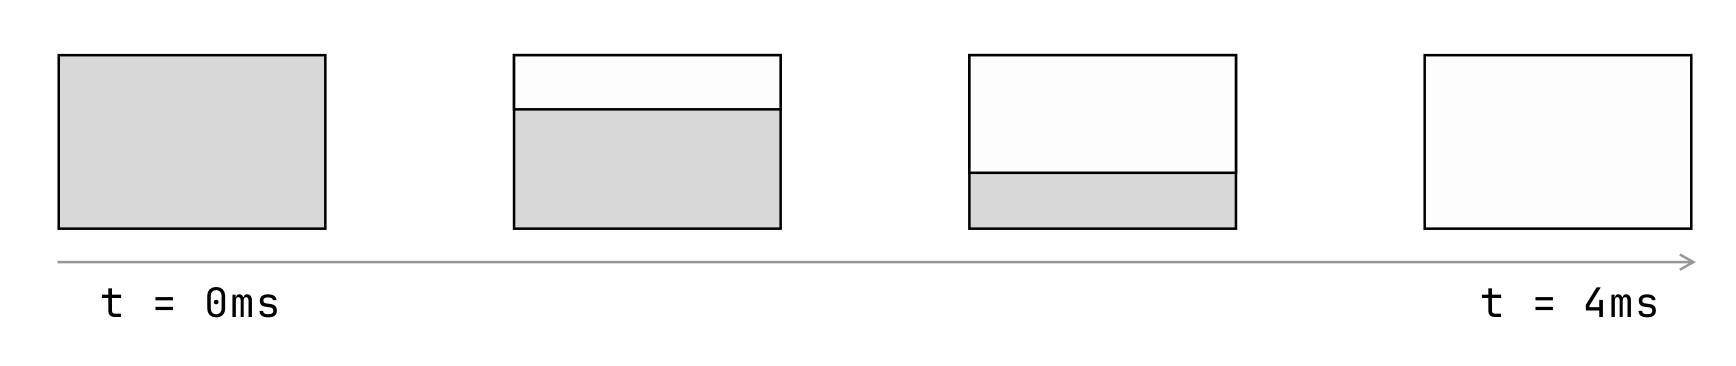
\includegraphics[width=0.55\linewidth]{assets/20260810-1.png}
\end{center}

Separately, the camera has a \emph{shutter speed}: how long the shutter stays open to collect light.  Unlike the readout time, the shutter speed is something the photographer freely chooses for each shot.  So there are two distinct restrictions on how long the sensor gathers light --- the readout time (a fixed property of the hardware) and the shutter speed (a setting you pick).

A flash, however, fires for an extremely brief instant.  For the flash to illuminate the whole frame evenly, every row of the sensor must be exposing at the same instant, so the shutter must stay open long enough for the entire rolling-shutter sweep to finish.  This minimum requirement is exactly the readout time.

The \emph{flash synchronization speed} is the fraction $1/N$ numerically equal to the readout time.  This is intuitive: your flash must be on for the entire time your sensor is collecting data.  Despite the name ``speed,'' it is not a speed in the physical sense; it is a time interval.  For example, a sensor whose readout time is $4\,\mathrm{ms}$ has a flash sync speed of $1/250\ \mathrm{s}$, because $1/250\ \mathrm{s} = 4\,\mathrm{ms}$.  Your flash must therefore be on for $1/250\ \mathrm{s}$ if your camera needs $4\,\mathrm{ms}$ to collect data across the sensor.

\emph{Lemma (illuminated fraction).}  Because the wavefront travels at a constant rate, the illuminated fraction of the sensor is proportional to the exposure time.  If the shutter is open for a time less than the sync time, then the fraction of the sensor that receives the flash is
\[
\boxed{\ \frac{\text{shutter speed}}{\text{flash sync speed}} \ }.
\]
For example, a shutter speed of $1/1000\ \mathrm{s}$ on a $1/250\ \mathrm{s}$ sensor illuminates only
\[
\frac{1/1000}{1/250} = \frac{1}{4} = 25\%
\]
of the sensor.

Equivalently, if $s$ is the \emph{height} of the band already swept, then
\[
\boxed{\ s(t) \propto t \ }.
\]
This is the same statement in disguise: the swept height at the flash instant is $s(t^{*}) = 24\,\mathrm{mm} \times \dfrac{\text{shutter speed}}{\text{flash sync speed}}$.

To make this precise, let $S(t)$ be the region of the sensor that has already been scanned at time $t$.  Model the sensor as a $36\,\mathrm{mm} \times 24\,\mathrm{mm}$ rectangle in the $(x,y)$-plane, with the readout wavefront sweeping downward from the top edge $y = 24$:
\[
  S(t) = \{\, (x, y) \;:\; 0 \le x \le 36,\;\; 24 - s(t) \le y \le 24 \,\},
\]
where $s(t)$ is the height of the band already swept.  Since the wavefront moves at constant speed, $s(t) \propto t$; consequently the scanned area also grows linearly, $\int_{S(t)} \dd A = 36\,\mathrm{mm} \cdot s(t) \propto t$.  At the readout time the whole sensor has been swept, $s(\text{readout}) = 24\,\mathrm{mm}$ and $\int_{S(\text{readout})} \dd A = 36 \times 24\ \mathrm{mm}^{2}$.  The flash fires at the instant $t^{*} = \min(\text{shutter speed}, \text{flash sync time})$; the band already swept at that instant is the illuminated region.

In practice this means photographers rarely think about the readout time at all.  It is a fixed hardware number whose only visible consequence is the flash sync speed --- a ceiling on how fast a shutter speed can be used with flash.  So most of the time we only care about the shutter speed, because the readout speed merely limits the range of shutter speeds available to us.

Now Jason runs a lab.  He cuts out two pieces of paper: one enclosed by the region
\[
  0 \le x \le 20\,\mathrm{mm},
  \qquad
  -\frac{x^{2}}{100} \le y \le \frac{x^{2}}{100},
\]
and the other a circle of radius $10\,\mathrm{mm}$.

\begin{center}
  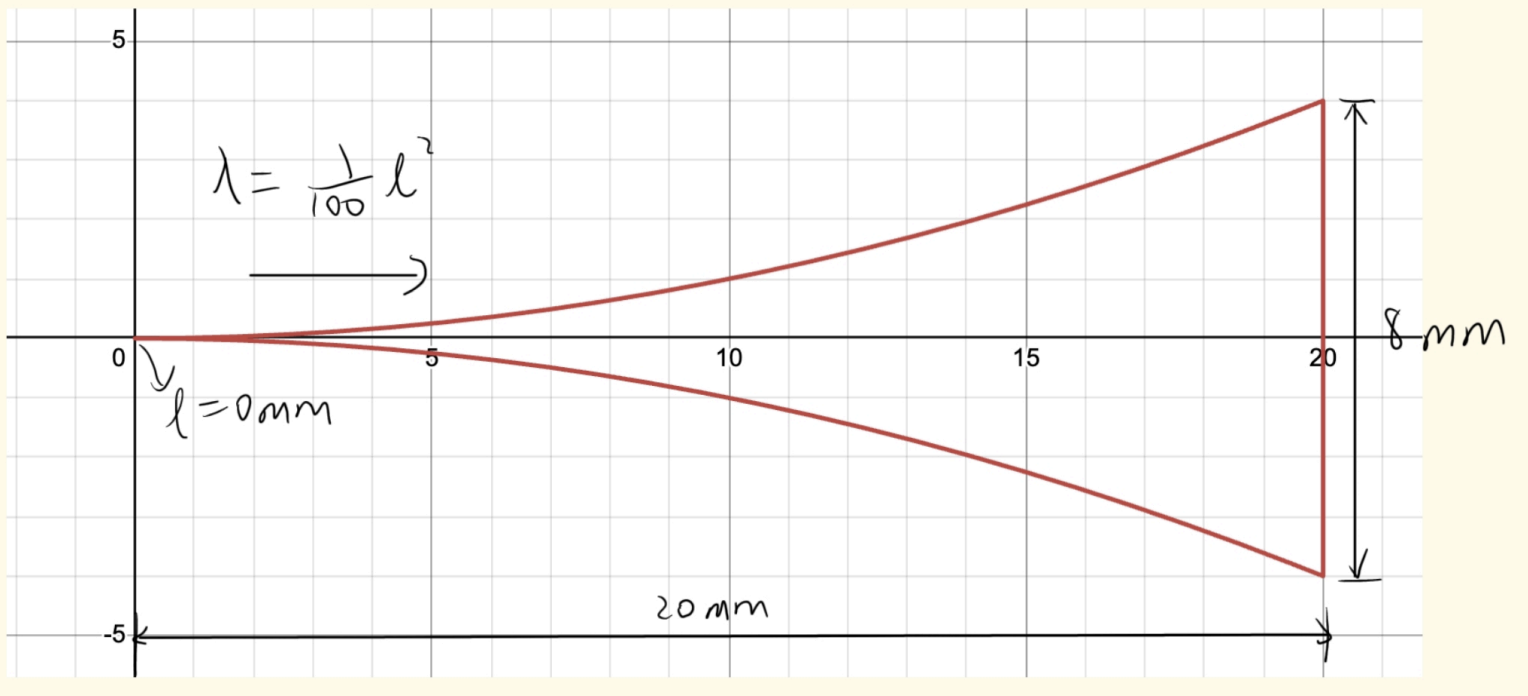
\includegraphics[width=0.55\linewidth]{assets/20260810-2.png}
\end{center}

He places them on a board as shown:

\begin{center}
  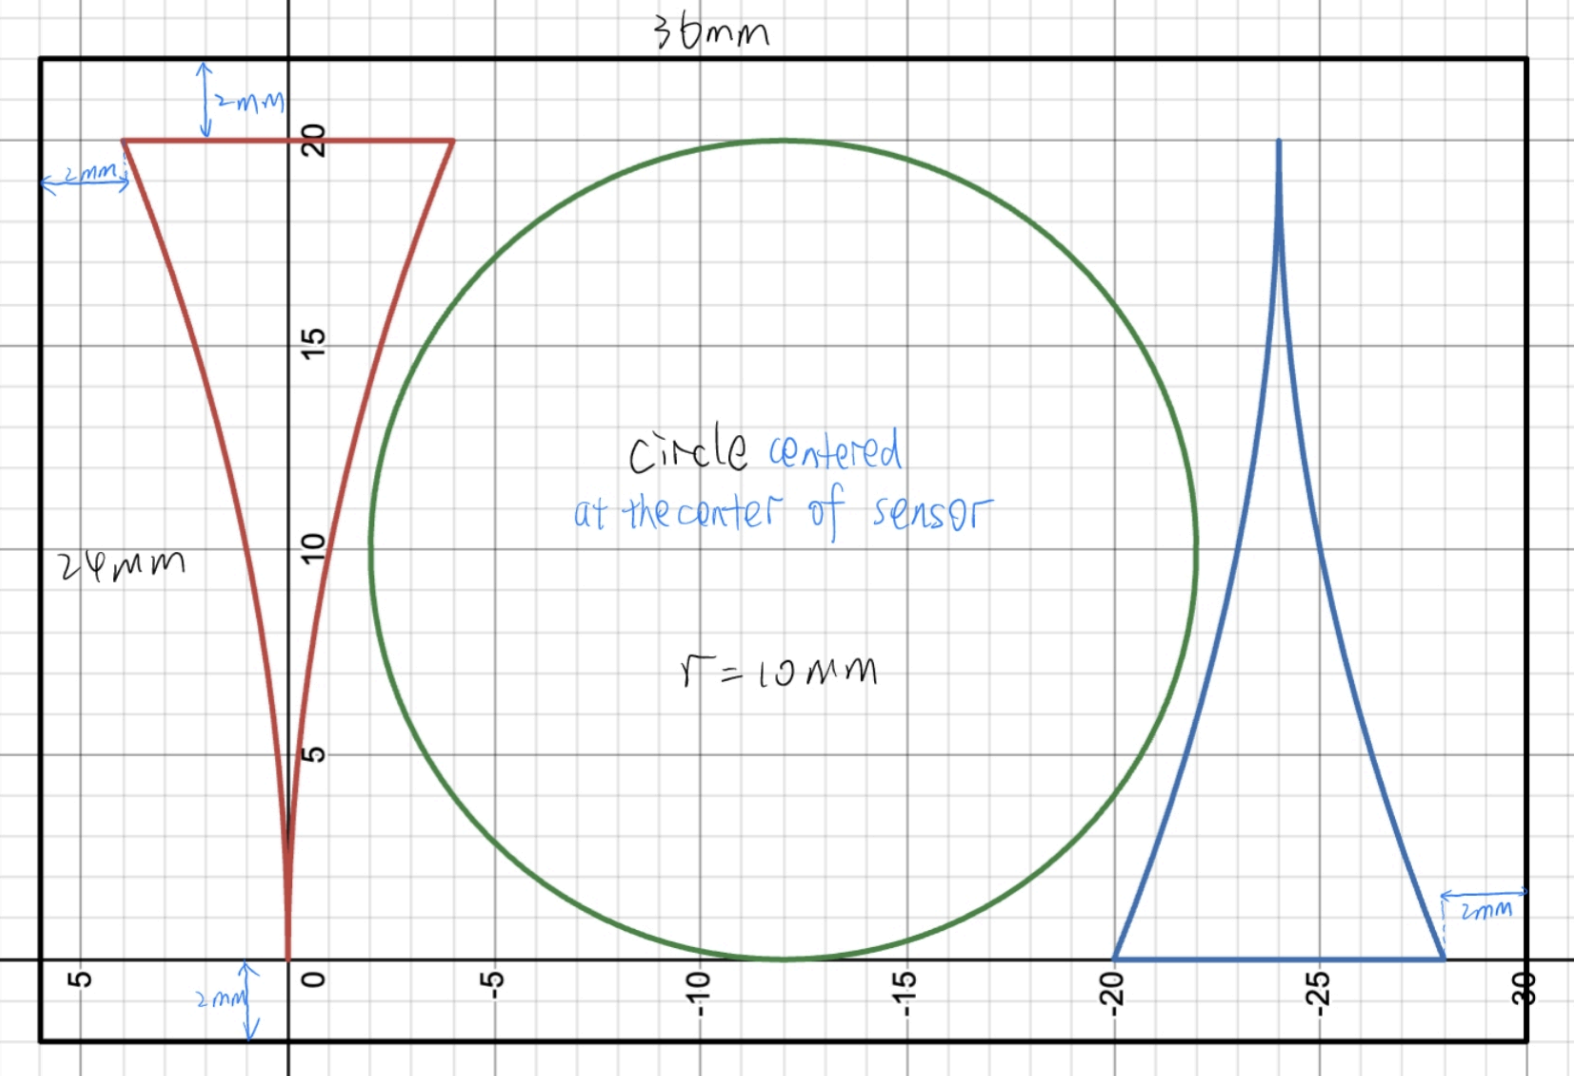
\includegraphics[width=0.55\linewidth]{assets/20260810-3.jpg}
\end{center}

and photographs the board through a $1\times$ macro lens.  This means everything is projected $1{:}1$ onto the sensor --- every millimetre on the paper maps to one millimetre on the sensor.

For the Canon EOS R6 Mark II used here, the readout time is $14.73\,\mathrm{ms}$ --- equivalently, its flash sync time is $14.73\,\mathrm{ms}$.  Jason sets his shutter speed to $1/200\ \mathrm{s}$.

\begin{questions}
  \item \textbf{Illuminated area.}
        Derive the area of the pieces of paper that are actually illuminated by the flash.  That is, evaluate
        \[
          \int_{S(t^{*})\,\cap\,\text{paper}} \dd A,
          \qquad
          t^{*} = \min(\text{shutter speed},\ \text{flash sync time}).
        \]
\end{questions}

\end{problem}

\begin{solution}{20260810}

\subsection*{Q1. Illuminated Area}

\textbf{Step 1: the swept height.}  Flip the sensor upside down so the illuminated band sits at the top.  By the illumination lemma,
\[
s(t^{\ast}) = 24\,\mathrm{mm}\times\frac{\text{shutter speed}}{\text{flash sync time}}
           = 24\,\mathrm{mm}\times\frac{1/200\ \mathrm{s}}{14.73\,\mathrm{ms}}
           = 24\times\frac{5}{14.73}
           \approx 8.147\,\mathrm{mm}.
\]

\textbf{Step 2: the paper's vertical extent.}  Both pieces are elevated $2\,\mathrm{mm}$ off the board, and the disk of radius $10\,\mathrm{mm}$ centred at $y = 12$ also has its lowest point at $y = 2$.  Hence the paper occupies $y \in [2,\,22]$, and its overlap with the illuminated band $[0,\,8.147]$ is
\[
  y \in [\,2,\ 8.147\,].
\]

\textbf{Step 3: integrate.}  At each height $y$, the horizontal width of a strip is proportional to the square of its distance from the thin tip, so the three contributions are:

\emph{Strip 1 (broad head down).}  Width $\dfrac{(22-y)^{2}}{50}$:
\[
  A_{1} = \int_{2}^{8.147} \frac{(22-y)^{2}}{50}\,\dd y
        = \frac{(20)^{3}-(22-8.147)^{3}}{150}
        \approx 35.61\ \mathrm{mm}^{2}.
\]

\emph{Strip 2 (thin head down).}  Width $\dfrac{(y-2)^{2}}{50}$:
\[
  A_{2} = \int_{2}^{8.147} \frac{(y-2)^{2}}{50}\,\dd y
        = \frac{(8.147-2)^{3}}{150}
        \approx 1.55\ \mathrm{mm}^{2}.
\]

\emph{Disk.}  Width $2\sqrt{100-(y-12)^{2}}$:
\[
  A_{3} = \int_{2}^{8.147} 2\sqrt{100-(y-12)^{2}}\,\dd y
        \approx 81.96\ \mathrm{mm}^{2}.
\]
(The antiderivative is $(y-12)\sqrt{100-(y-12)^{2}}+100\arcsin\frac{y-12}{10}$; the numeric value follows from a CAS.)

\textbf{Total illuminated area:}
\[
  \boxed{A = A_{1}+A_{2}+A_{3} \approx 35.61 + 1.55 + 81.96
           = 119.1\ \mathrm{mm}^{2}}.
\]

\end{solution}

\input qpd-end
